\documentclass[a4paper]{article}

%%%%%%%%%%%%%%%紙張大小設定%%%%%%%%%%%%%%%
% \paperwidth=65cm
% \paperheight=160cm

%%%%%%%%%%%%%%%引入Package%%%%%%%%%%%%%%%
\usepackage[margin=3cm]{geometry} %上下左右距離邊緣2cm
\usepackage{amsmath,amsthm,amssymb} % 引入 AMS 數學環境
\usepackage{graphicx}    %圖形插入用
\usepackage{fontspec}    %加這個就可以設定字體
\usepackage{titlesec}   %設定section等的字體
\usepackage{titling}    %加強版title
\usepackage{fancyhdr}   %頁首頁尾
%\usepackage{sectsty}	%設定section的字體
\usepackage{type1cm}	%設定fontsize用
\usepackage{tabularx}   %加強版 table
\usepackage{multirow}   %表格 multirow
\usepackage{array}      %
\usepackage{listings}	%insert code
\usepackage{subfigure}  %using subfigure
\usepackage[square, comma, numbers, super, sort&compress]{natbib}
%cite加強版
\usepackage[unicode=true, pdfborder={0 0 0}, bookmarksdepth=-1]{hyperref}
%ref加強版

\usepackage[AutoFakeBold, CheckSingle, CJKmath]{xeCJK}
%讓中英文字體分開設置
%\usepackage{zhspacing}
\usepackage{soul}       %highlight
\usepackage{ulem}       %字加裝飾
\usepackage{CJKulem}	%中文字裝飾
\usepackage[usenames, dvipsnames]{color}%可以使用顏色
\usepackage{framed}     %可以加文字方框
\usepackage{enumerate}  %加強版enumerate
%\setmainfont{}          %設定字體,若無設定為原Tex字型
\newfontfamily\codefont[]{Source Code Pro}
%設定一小段字體 使用時用 \begin{myfont},\end{myfont}
\setCJKmainfont{BiauKai}
%設定中文為系統上的字型,而英文不去更動,使用原TeX字型
\setCJKsansfont{BiauKai}
\setCJKmonofont{BiauKai}
%\XeTeXlinebreaklocale "zh"             %這兩行一定要加,中文才能自動換行
%\XeTeXlinebreakskip = 0pt plus 1pt     %這兩行一定要加,中文才能自動換行
%\graphicspath{{images/}}  %搜尋圖片目錄
%\setcounter{secnumdepth}{4}  %章節標號深度

%%%%%%%%%%%%%%%字體大小設定%%%%%%%%%%%%%%%
\def\normalsize{\fontsize{12}{18}\selectfont}
%\def\large{\fontsize{40}{60}\selectfont}
%\def\Large{\fontsize{50}{75}\selectfont}
%\def\LARGE{\fontsize{90}{20}\selectfont}
% \def\huge{\fontsize{34}{51}\selectfont}
% \def\Huge{\fontsize{38}{57}\selectfont}

%%%%%%%%%%%%%%%
%針對中文數字(壹貳參...etc.)定義,section等標號,eq等編號
%%%%%%%%%%%%%%%
\newcommand{\BCJKcount}[1]{\ifcase #1\or 壹\or 貳\or 參\or 肆\or 伍
                                     \or 陸\or 柒\or 捌\or 玖\or 拾\else\fi}
\newcommand{\CJKcount}[1]{\ifcase #1\or 一\or 二\or 三\or 四\or 五
                                    \or 六\or 七\or 八\or 九\or 十\else\fi}
\newcommand{\SCJKcount}[1]{\ifcase #1\or (一)\or (二)\or (三)
                                     \or (四)\or (五)\or (六)
                                     \or (七)\or (八)\or (九)
                                     \or (十)\else\fi}

%\titleformat{\section}{\centering\Large}
            %{\BCJKcount{\arabic{section}}、}{0em}{}
%\titleformat{\subsection}{\large}
            %{\CJKcount{\arabic{subsection}}、}{0em}{}
%\titleformat{\subsubsection}{\bf\normalsize}
            %{\SCJKcount{\arabic{subsubsection}}、}{0em}{}
%\titleformat{command}[shape]{format}{label}
            %{編號與標題距離}{before}[after]

%\numberwithin{equation}{section}

%%%%%%%%%%%%%%%頁面設定%%%%%%%%%%%%%%%
\setlength{\droptitle}{-1.5cm} %title 與上緣的間距
\parindent=24pt %設定縮排的距離
%\pagestyle{empty}  %去除頁碼
%\parskip=1ex  %設定行距

\pagestyle{fancy}  %強化頁首頁尾
%\parskip=1ex  %設定行距

%use with fancygdr
\lhead{\leftmark}
\chead{}
\rhead{}
\lfoot{Author:陳奐廷}
\cfoot{}
\rfoot{\thepage}
\renewcommand{\headrulewidth}{0.4pt}
\renewcommand{\footrulewidth}{0.4pt}
%\fancypagestyle{firststyle}
%{
   %\fancyhf{}
   %\fancyfoot[C]{\footnotesize Page \thepage\ of \pageref{LastPage}}
%}

%%%%%%%%%%%%%%%重定義一些command%%%%%%%%%%%%%%%
\renewcommand{\contentsname}{目錄}  %設定目錄的標題名稱
\renewcommand{\refname}{參考資料}  %設定參考資料的標題名稱
\renewcommand{\abstractname}{\LARGE Abstract} %設定摘要的標題名稱

%%%%%%%%%%%%%%%特殊函數符號設定%%%%%%%%%%%%%%%
%\newcommand{\citet}[1]{\textsuperscript{\cite{#1}}}
\newcommand{\np}[1]{\\[{#1}] \indent}
\newcommand{\transpose}[1]{{#1}^\mathrm{T}}
\newcommand{\per}{\mbox{per}}

%%%%%%%%%%%%%%%證明、結論、定義等等的環境%%%%%%%%%%%%%%%
\renewcommand{\proofname}{\bf 證明:} %修改Proof 標頭
\newtheoremstyle{mystyle}% 自定義Style
  {6pt}{15pt}%       上下間距
  {}%               內文字體
  {}%               縮排
  {\bf}%            標頭字體
  {.}%              標頭後標點
  {1em}%            內文與標頭距離
  {}%               Theorem head spec (can be left empty, meaning 'normal')
%%%%%%%%%%%%%% code setting %%%%%%%%%%%%%%%%%
\lstdefinestyle{mystyle}{ %this is the stype
        frame=TB,
        numbers=left, 
        numberstyle=\small,
        basicstyle=\small, 
        keywordstyle=\color{black}\bfseries,
        otherkeywords={SDL_Rect, SDL_Rect*, SDL_Texture*, SDL_Thread*},
        xleftmargin=.04\textwidth,
        breaklines=true,
        showstringspaces=false,
		captionpos=b
        }
\lstset{style=mystyle,language=C++}

% 改用粗體,預設 remark style 是斜體
\theoremstyle{mystyle}	% 定理環境Style
\newtheorem{thm}{Theorem}
\newtheorem{dfn}{Definition}
\newtheorem{formula}{Formula}
\newtheorem{cdn}{Condition}
\newtheorem{pbm}{Problem}
\newtheorem{ex}{Example}
\newtheorem{lem}{Lemma}
\newtheorem{pty}{Property}
\newtheorem{cor}{Corollary}



%%%%%%%%%%%%%%%Title的資訊%%%%%%%%%%%%%%%
\title{BoomBoomKing} %標題
\author{陳奐廷} %作者
\date{\today} %不要日期

\begin{document}
\maketitle %製作title page
\thispagestyle{fancy}  %使用fancyhdr
%\tableofcontents %目錄
\setcounter{section}{-1} %設定section起始數字
%%%%%%%%%%%%%%%%%%%%%%%%%%%%%%%%%%%%%%%%%%%%%%%%%%%%%%%%%%%%%
\section{遊戲簡介}
BoomBoomKing這款遊戲,是以知名遊戲「爆爆王」為藍圖,再增加一些功能,綜合所得的一款兩個玩家對戰的遊戲。遊戲的目標是把敵方炸死。每個玩家可以下炸彈(不限顆數),以及地雷(限兩顆)。地圖上一開始會有道具,之後每隔一段時間會產生新的道具。道具有兩個:超級炸彈以及無敵藥水。當你吃到超級炸彈,你的炸彈所爆炸的範圍會變大;而無敵藥水的效果是不會被炸彈所炸死,但仍然無法逃過地雷。
\begin{figure}[ht]
\begin{center}
\graphicspath{{project_image/}}
\subfigure[main menu]{
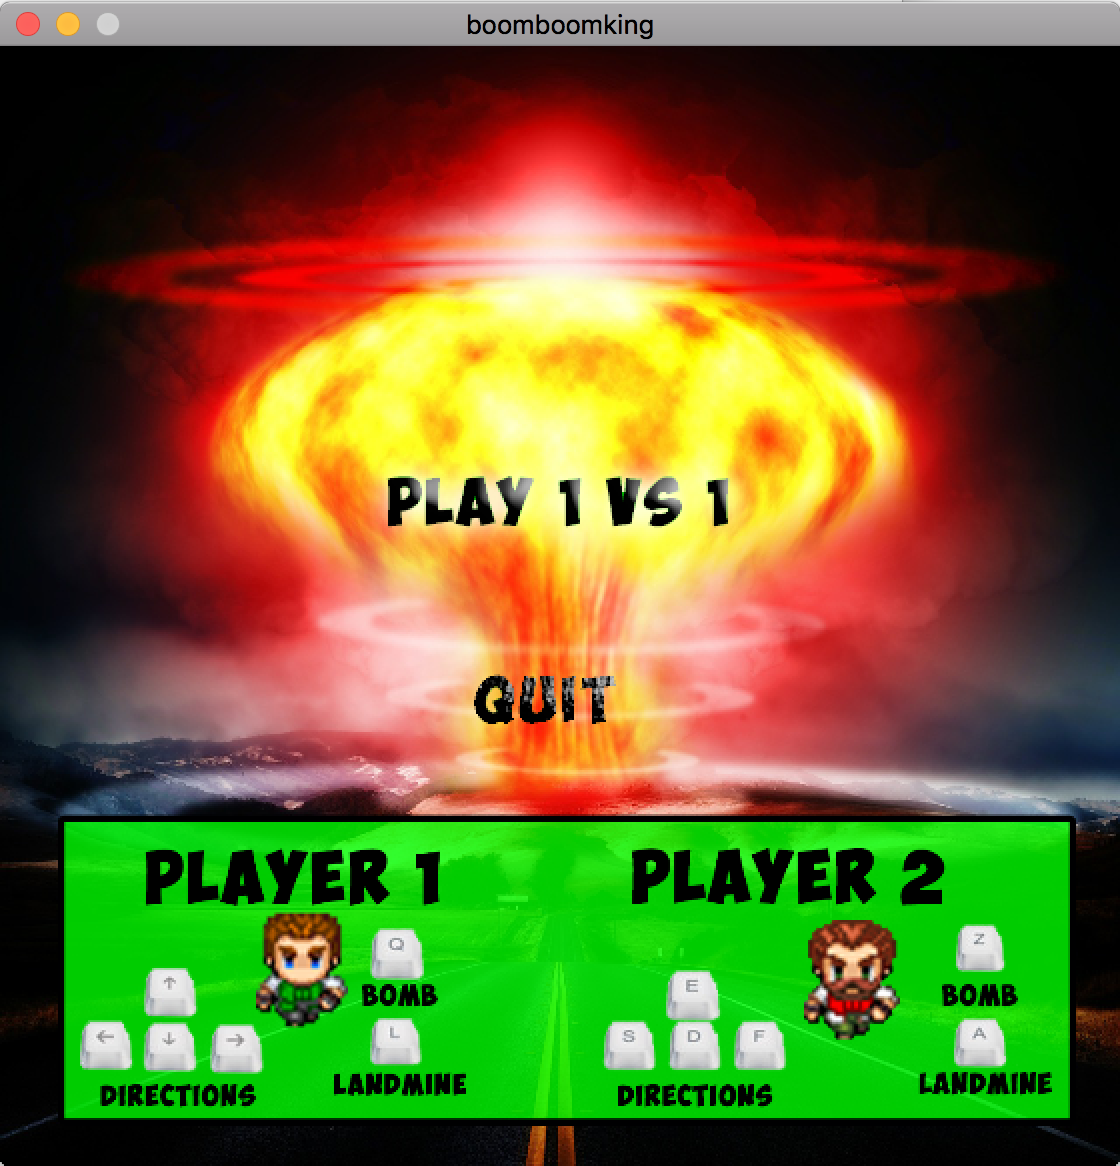
\includegraphics[width=0.4\textwidth]{main.png}}
\hspace{2em}
\subfigure[while playing]{
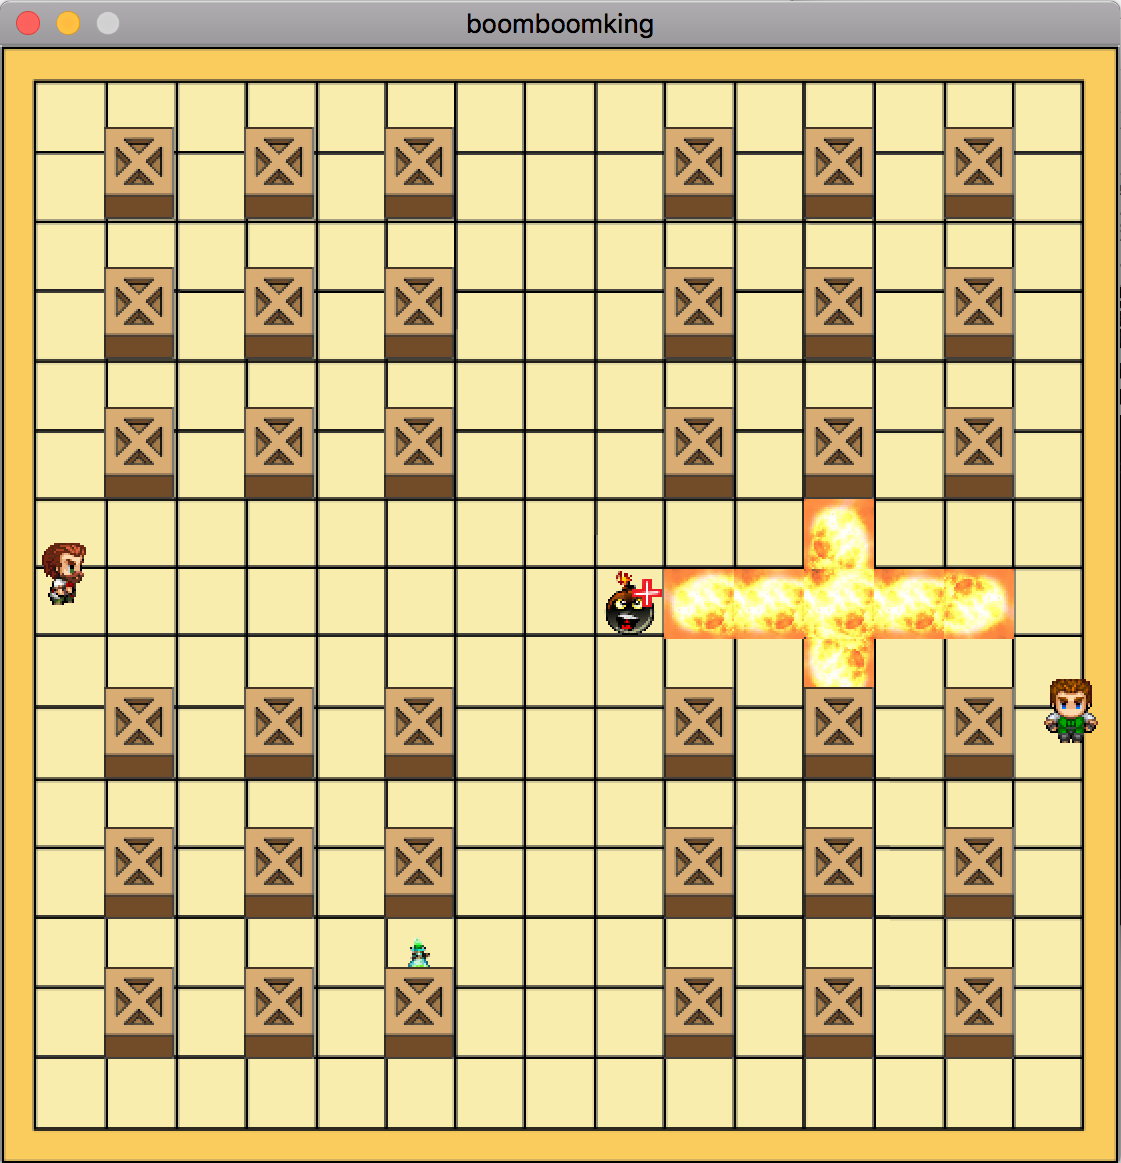
\includegraphics[width=0.4\textwidth]{playing.png}}
\caption{遊戲介面}
\end{center}
\end{figure}
\section{程式分工}
我們的專題使用了大量的class來實作,每個組員分別寫幾個不同的class,而最後是由我來彙整所有的檔案,再做一些必要的修改。這樣的好處是我的main.cpp檔裡面非常的乾淨,只有少數幾個函式而已,而且日後如果需要擴充功能,或是需要做一些調整都非常的方便。在這次的專題裡,我貢獻的檔案有 main.cpp, background.cpp, tools.cpp, landmine.cpp, show\_bomb.cpp, LTexture.cpp, 部分的characher.cpp(還有這些檔案相對應的.hpp檔)。
\section{Class實作}
以下舉的例子是我所寫的code裡,我覺得值得特別拿出來討論的部分。
\subsection{LTexture}
將Lazyfoo sample code 輸入圖檔的部分另外寫成一個class,再稍作修改,使之符合我們需要。在解構的部分,我們把解構的函式另外寫成一個函式{\codefont \small free()},方便之後使用。\\\\
\begin{codefont}
\begin{minipage}[c]{0.49\textwidth}
\begin{lstlisting}[xleftmargin=0.08\textwidth, caption={LTexture.hpp 18-49}]
class LTexture{
public:
    LTexture();  //constructor
    ~LTexture(); //destructor
    void free(); //deallocate function
    //omit some functions here
private:
    //omit some variable
    SDL_Texture* mTexture;
    int mWidth;
    int mHeight;
};

\end{lstlisting}
\end{minipage}%
\hfill
\begin{minipage}[c]{0.49\textwidth}
\begin{lstlisting}[xleftmargin=0.08\textwidth, caption={LTexture.cpp 23-27,71-81}]
LTexture::~LTexture(){
    free();
}
void LTexture::free(){
    if( mTexture != NULL )
    {
        SDL_DestroyTexture( mTexture );
        mTexture = NULL;
        mWidth = 0;
        mHeight = 0;
    }
}
\end{lstlisting}
\end{minipage}
\end{codefont}
\subsection{Background Class}
background class是為了輸出背景及障礙物所寫的class。包含了所有與輸出背景有關的函式,用{\codefont \small box\_rerendering }來解決人物與障礙物重疊的問題。\\
有寫constructor來初始化數值,不過在這個class沒有用到任何的指標,所以就不需要再另外寫destructor,直接用預設的就可以了。\\
\begin{codefont}
\begin{lstlisting}[caption={background.hpp 18-34}]
class Background{
private:
	//omit some variables here
public:
    Background(); //constructor
    bool loadMedia(); //loadMedia function
    void background_rendering(); //render the background
    void box_rendering(); //render the box
    void box_rerendering(int, int); //rerender boxes that overlap with the character
    bool check_character_behind_box(int, int);
    SDL_Rect blockwall[15][15];  //-----blockwall[y-axis][x-axis]
};
\end{lstlisting}
\end{codefont}
\subsection{Bomb Class}
\label{sec:bomb}
Bomb Class 是我認為封裝的最完整的一個class。
\begin{enumerate}
\item 有privite,public的區分,而且將所有與炸彈有關的函式全部寫進來,相當的完整。
\item 在{\codefont \small set\_bomb\_position}這個函式當中,以call by reference的方式,讓位置不會跑掉。
\item 在這個class中,沒有用destructor,取而代之的是寫一個解構的函式。是因為在主程式中,這個class是重複使用的,我不希望在執行結束之後馬上把這個class解構掉,所以在主程式的最後才呼叫{\codefont \small free()}把它解構掉。(其實就是因為加了destructor程式會有bug,經過無限的debug之後,發現把destructor拿掉就過了...)
\label{itm:dstr}

\end{enumerate}
\begin{codefont}
\begin{lstlisting}[caption={show\_bomb1.h 15-88}]
class Bomb{
private:
    //omit some variables and pointers here
public:
    Bomb();             //constructor
    void free();        //deallocate function
    enum bomb_index_number{  /*omit the enumeration*/  };
    enum KeyPressSurfaces{  /*omit the enumeration*/  };
    void set_bomb_position(double &,double &);
    void bomb_display(int, int);		//display bombs on the map
    SDL_Texture* texture_bomb;      //bomb texture declaration
\end{lstlisting}
\end{codefont}
\subsection{Character Class}
這個class中有一部分不是我主筆,但是有一大部分是我主筆的,另一部份我也有參與討論,故也放上來。
\begin{enumerate}
\item 在constructor的部分,因為要針對兩個不同的角色做不同的初始化,所以用\\{\codefont \small charachter(enum)}的方式來寫。雖然只有兩個角色,但是用enum寫的好處就是之後如果要新增更多角色,這樣再去更改會比較容易和美觀。
\item 在參數的設定上,有加上{\codefont \small const, static},這樣避免其他的函式不小心去修改到他的數值。其中有一個參數忘記加{\codefont \small const}雖然不會有問題但是我覺得還是不好。
\item {\codefont \small check\_Collision(SDL\_Rect, SDL\_Rect*)}是為了檢查角色有沒有撞到障礙物所寫的函式。因為障礙物是用15*15的陣列去存,所以我讓他傳入一個指標,就可以用一個兩層的迴圈,然後裡面放{\codefont \small temp[i][j] = *(b+15*i+j);}。
\item 我有重新定義一個operator= ,因為在建立contructor的時候,同樣argument數的建構式有不只一個,所以他的operator=會不能用,需要重新定義成default。不過後來主程式需要用到這個的部分改掉了,所以我把這個operator註解掉了。
\end{enumerate}
\begin{codefont}
\begin{lstlisting}[caption={Charachter.hpp 20-105}]
enum player{  /*omit the enumeration*/  };
class Charachter{
private:
    //omit some variables and pointers here
    const int WALKING_ANIMATION_FRAMES = 3; //parameter setting
    int WALKING_ANIMATION_SIZE = 32;    //parameter setting (adding 'const' in the front should be better but i forgot orz)
public:
    static const int CHAR_WIDTH = 32;   //parameter setting
    static const int CHAR_HEIGHT = 32;  //parameter setting
    static const double CHAR_VEL = 1;	//parameter setting
    Charachter(enum player playable);	//different constructors for each character(player)
    bool checkCollision( SDL_Rect, SDL_Rect* );    //check collision between character and obstacles
    Charachter& operator= (const Charachter& a) = default; //this line is commented in the file
};
\end{lstlisting}
\end{codefont}
\section{其他程式細節}
以下介紹一些主程式碼中,我覺得還蠻有巧思的地方,以及我debug很久的地方。
\subsection{Thread}
因為程式的需要,我必須讓主程式運作的同時,也做其他事情。例如說炸彈引爆的連續動作中,角色必須繼續移動。所以我需要同時平行的去執行一些程式碼,也就是利用Thread來增加執行序。C++中有內建的<thread>可以用,不過在專題裡,我是使用SDL Library裡的thread功能。
\subsection{Bomb Declaration}
在遊戲裡,玩家可以放置炸彈的數量是無上限的,而每一顆炸彈都是一個新的class,所以我開了一個陣列{\codefont \small bomb\_array[MAX\_BOMB]}來存每一個bomb class。{\codefont \small MAX\_BOMB}是同時可以存在的炸彈個數,我用define去定義它對於之後要改參數會比較方便。當數量超過{\codefont \small bomb\_array[MAX\_BOMB]}時,會把第一顆取代掉。同理也有一個{\codefont \small bomb\_showing\_threads[MAX\_BOMB]}讓每一個bomb都有一個thread。這應該也是造成在{\color{blue}\ref{sec:bomb}}節中第{\color{blue}\ref{itm:dstr}}點裡提到的加上destructor會有bug的原因:我有可能還會重複使用第一個bomb class,所以當第一個bomb class執行完,我仍然不能解構它,要保留他的位置。\\
有個值得一提的點是,我一開始並不是用array去存bomb class,我是用vector去存。我認為vector能夠自由伸縮長度,每多下一顆炸彈,就可以用{\codefont \small push\_back()}加在這個vector後面,比array自由許多。但是結果是出現很奇怪的bug:有一些炸彈很順利的執行,而有一些會有問題。debug很久之後才發現,問題出在vector運作的原理上面。vector會先給定一個預設大小的記憶體,當他已經滿了的時候,在新增一個物件進去,它會把整個vector搬到另一個地方,並且空間是前一個的兩倍大。當我某一個炸彈的thread做到一半,剛好進行這個搬移的動作,那存在原本那個位址的變數就整個跑掉導致有bug。\\
\begin{codefont}
\begin{lstlisting}[otherkeywords={Bomb, SDL_Thread*}, caption={main.cpp 71-75, 234-245}]
#define MAX_BOMB 50
Bomb bomb_array[MAX_BOMB]={};   //bombs array (allowing to show MAX_BOMB bombs at the same time)
SDL_Thread* bomb_showing_threads[MAX_BOMB];   //threads array
if(e.key.keysym.sym==SDLK_l){
    double x = charachter1.getposx(), y=charachter1.getposy();
    Bomb a;
    a.bomb_character=1;
    if( !a.loadMedia() ) { printf( "Failed to load bombs media!\n" );}
    else{
        bomb_array[count % MAX_BOMB] = a;
        bomb_array[count % MAX_BOMB].set_bomb_position(x,y);
        bomb_showing_threads[count % MAX_BOMB] = SDL_CreateThread( show_bomb_thread, "show_bomb",(void*)(bomb_array+(count %  MAX_BOMB)));   //creating thread for each bomb
        count++;
    }
}
\end{lstlisting}
\end{codefont}
\subsection{Close}
\label{sec:close}
\begin{minipage}[c]{0.35\textwidth}
在主程式的最後有一個{\codefont \small close()}函式。裡面充斥著{\codefont \small free()}函式(之前沒有把它解構掉的東西現在才來解構)和一些SDL相關的關閉視窗,讓程式順利結束。
\end{minipage}
\hfill
\begin{minipage}[c]{0.6\textwidth}
\begin{codefont}
\begin{lstlisting}[caption={main.cpp 576-610}]
void close(){
    for(int i=0;i<MAX_BOMB;i++){
        bomb_array[i].free();
    }
    SDL_DestroyRenderer( gRenderer );
    gRenderer = NULL;
    SDL_DestroyWindow( gWindow );  //Destroy window
    gWindow = NULL;
    IMG_Quit();    //Quit SDL subsystems
    SDL_Quit();
}

\end{lstlisting}
\end{codefont}
\end{minipage}
\section{奇聞軼事}
多人一起在寫程式的時候,往往會出現一些bug。有一些bug雖然需要de很久,但是至少是已知的bug。而有一些真的就非常的神奇,至今仍然未解。
\subsection{神奇的13月}
我的Mac是High Sierra最新版,Xcode也有更新到最新,但是只要用到SDL Library,就會有bug。編譯會過,但是執行出來第一行會顯示:Month 13 is out of bounds,然後就無法繼續執行下去。所以我只好改開terminal用g++編譯,就可以正確執行。我猜測是跟之前Apple出大bug(iphone時間壞掉,全部當機)一樣的原因,可是到現在仍然不能用。
\subsection{神奇的Mac\&Windows}
Mac和Windows的作業系統不知道為什麼也會有神奇的差異。
\subsubsection{神奇的const}
剛開始做專題就發現了這個問題:所有在Mac上的code丟到windows去都不能編譯。後來才發現是因為Xcode的預設檔案裡,是用{\codefont \small int main()(int argc, const char * argv[])},然後要把{\codefont \small const}刪掉,才可以在windows系統順利執行。
\subsubsection{神奇的編譯結果}
全部寫完專題的時候發現,用一模一樣的code,但是在兩個系統底下會產生不一樣的結果。
\begin{enumerate}
\item 在Mac底下完全可以正常運作的code,用windows下會停止運作。問題出在於第{\color{blue}\ref{sec:close}}節講到的{\codefont \small close()}函式。在專題截止死線前夕,我才忽然發現在windows系統底下會出事,所以只好把那段函式註解掉一部份,才可以順利執行。
\item 在兩個系統底下執行出來的結果不一樣。在人物死掉的時候,在Mac系統底下,爆炸火花會閃,如demo影片裡大約4:24-4:29, 4:40-4:45等片段所拍的。參見({\color{blue}www.youtube.com/watch?v=XMvianJXzWo})。可是在windows系統底下跑,卻不會有這樣的現象發生。
\end{enumerate}
\begin{figure}[ht]
\begin{center}
\graphicspath{{project_image/}}
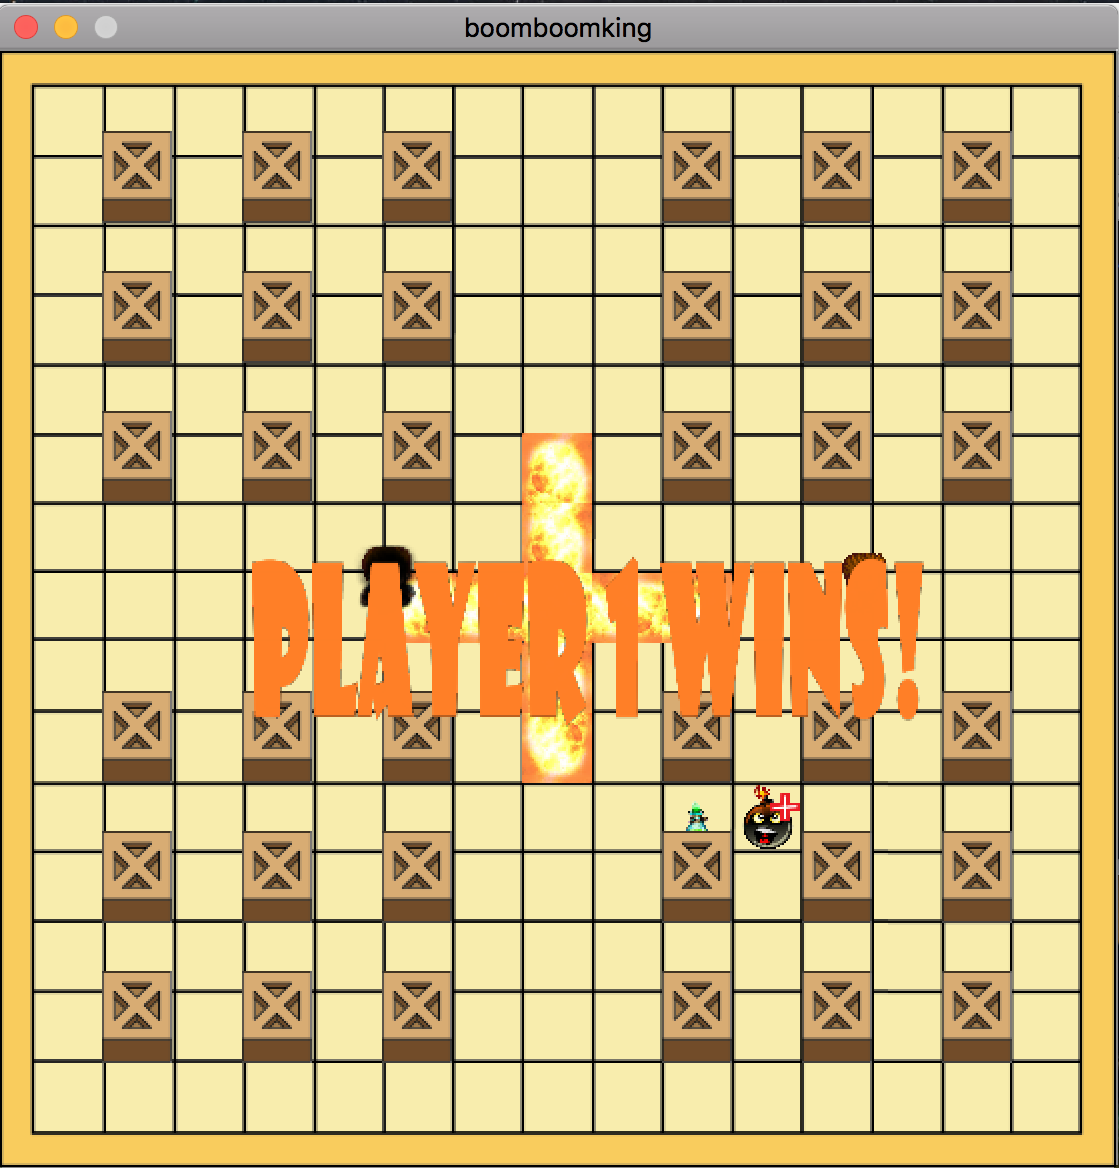
\includegraphics[width=0.35\textwidth]{player1win.png}
\hspace{2.5em}
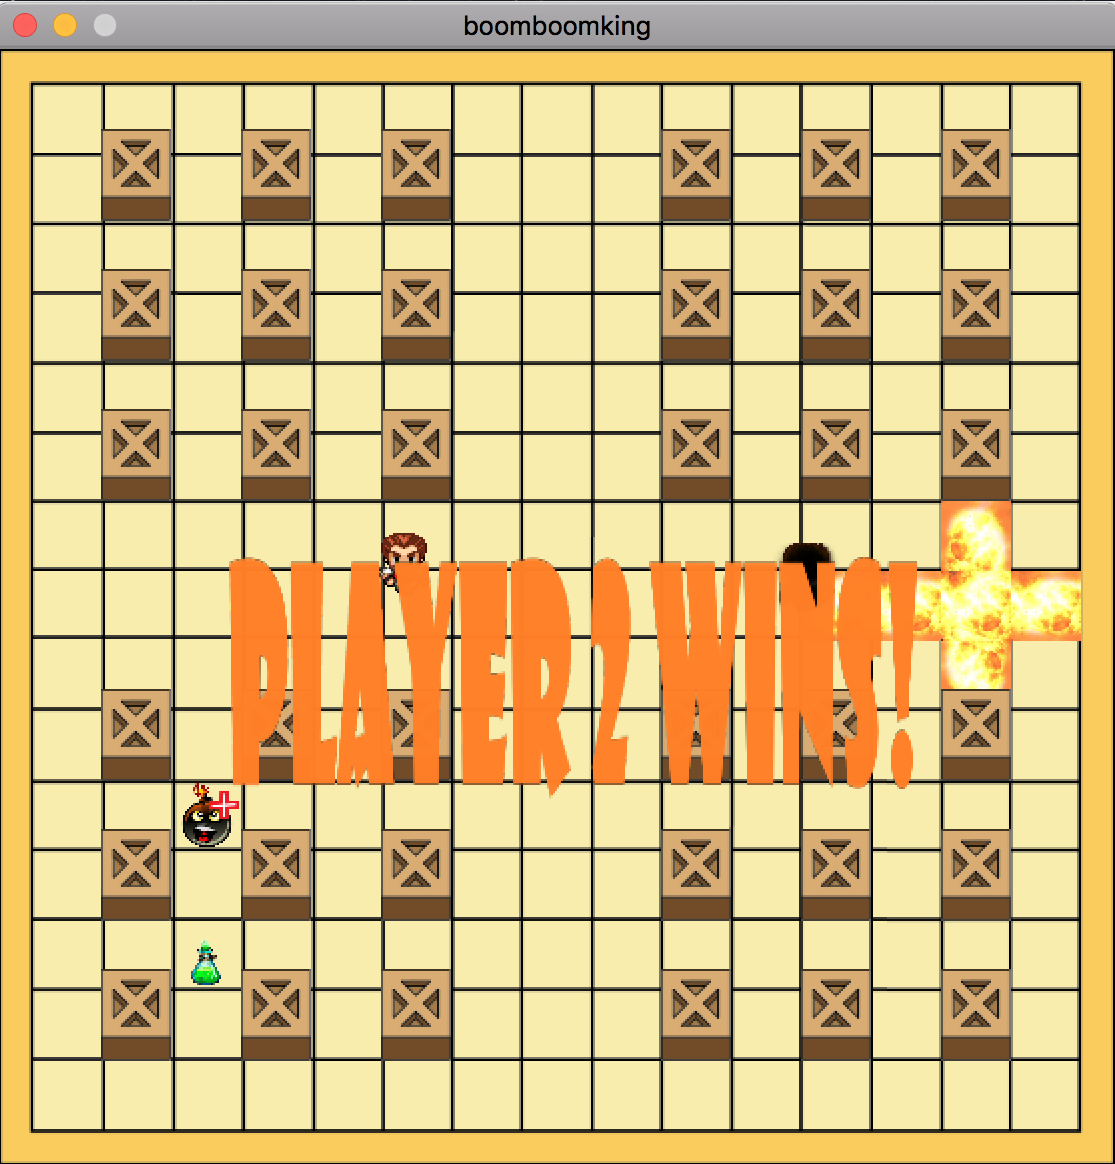
\includegraphics[width=0.35\textwidth]{player2win.png}
\end{center}
\end{figure}







%%%%%%%%%%%%%%%%%%%%%%%%%%%%%%%%%%%%%%%%%%%%%%%%%%%%%%%%%%%%%
%\begin{thebibliography}{99}
%\bibitem[]{}
%\end{thebibliography}
\end{document}
